La gestione della persistenza \`e un argomento delicato nella progettazione di applicazioni software.
Lo sviluppo di applicazioni Object-Oriented che utilizzano un DBMS relazionale per immagazinare i dati in memoria secondaria \`e uno scenario molto comune. Ci\`o che rende complessa la costruzione dello strato di persistenza \`e il problema dell'\emph{object/relational impedence mismatch}, ovvero la discrepanza tra il paradigma Object-Oriented e il paradigma relazionale.\\
Fondamentalmente, gli oggetti fanno riferimento ad altri oggetti e perci\`o danno forma ad un grafo, a differenza degli gli schemi relazionali, che hanno invece una struttura tabellare e basati sull'algebra relazionale che definisce insiemi di tuple. La conversione di tuple in strutture a grafo spesso richiede molto tempo e pu\`o risultare difficile, infatti, viene anche descritta "\emph{Vietnam of Computer Science}".
Questo problema pu\`o esser diviso in pi\`u parti:
\begin{itemize}
\item \textbf{Struttura, Ereditariet\`a, Interfaccia e Polimorfismo}:\\
Una classe specifica gli attributi e i metodi che devono avere gli oggetti che appartengono ad essa e pu\`o anche far parte di una gerarchia (concetto di ereditariet\`a).
Il modello relazionale non contempla il concetto di “classe” di oggetti e non fornisce una analogia per le gerarchie, interfacce e polimorfismo.  
\item \textbf{Granularit\`a dei tipi di dato}:\\
Tipi di dati composti sono tipicamente  rappresentati nei linguaggi OO mediante classi di oggetti, mentre nel modello relazionale non si prevede alcun meccanismo per la definizione di tipi di dato composti. 
\item \textbf{Incapsulamento}:\\
Lo stato di un oggetto \`e incapsulato ed \`e accessibile attraverso i metodi. Lo stato di una riga di una tabella non contempla questo aspetto e pu\`o essere modificato in maniera diretta.
\item \textbf{Identit\`a}:\\
Gli oggetti esistono indipendentemente dal loro stato. Essi possono essere identici o uguali. Se due oggetti sono identici, essi sono lo stesso oggetto. Se sono uguali, essi contengono gli stessi valori. Nel modello relazionale, invece, le righe sono identificate solo dai valori che esse contengono.
\item \textbf{Associazioni}:\\
Il modello relazionale contempla solo un tipo di associazione: l'utilizzo di una chiave esterna, che si riferisce ad una chiave primaria di un'altra tabella. Il paradigma Object-Oriented contempla diverse tipologie di associazione: uno a uno, uno a molti, molti a molti.
\item \textbf{Coesione}:\\
Tutte le propriet\`a di un oggetto sono contenuto all'interno di esso. Invece, le relazioni che corrispondono ad una stessa entit\`a possono essere stati suddivisi in pi\`u tabelle (fase di ristrutturazione dello schema logico)
\end{itemize}
Il problema dell'impedence mismatch deve essere analizzato e risolto nel modo opportuno in fase di progettazione. 

Un altro aspetto molto importante nella gestione della persistenza \`e l'interazione tra lo strato di business logic e lo strato di persistenza.
In applicazioni Java la comunicazione con la base di dati avviene utilizzando API specifiche come ODB (Open Database Connectivity) o JDBC(Java Database Connectivity). 
Una delle strategie pi\`u valide e utilizzate \`e l'uso del pattern Data Access Object (DAO) per la creazione di oggetti che costituiscono uno strato di comunicazione con la base di dati. 
La realizzazione dei DAO avviene usando API JDBC
per rendere disponibili le operazioni CRUD(Create Read Update Delete) allo strato di logica applicativa. I DAO incapsulano l'accesso alla base di dati e permettono di gestire la maggior parte degli scenari ma la loro realizzazione necessita di una conoscenza dettagliata della base di dati.
Altri strategie fanno uso della serializzazione, di object oriented database systems oppure dell'Object-Relational Mapping che consiste nel mappare le classi di dominio dell'applicazione su una base di dati relazionale. 

\subsection{Object/Relational Mapping}
L'Object/Relational Mapping (ORM) \`e una tecnica di programmazione che favorisce l'integrazione di sistemi software aderenti al paradigma della programmazione orientata agli oggetti con sistemi RDBMS.
Attraverso questo mezzo ogni oggetto viene reso persistente nel database tramite l'inserimento di nuovi record i cui campi contengono i valori degli attributi dell'oggetto stesso. Si viene quindi a creare la relazione tra oggetto Java e tabella SQL. Una soluzione ORM consiste di quattro componenti caratteristici:

\begin{enumerate}
\item Una API per eseguire le operazioni CRUD sugli oggetti delle classi del modello.
\item  Un linguaggio  o una API  per specificare query che fanno riferimento alle classi e alle propriet\`a delle classi.
\item Uno srumento per la specifica del mapping mediante metadata.
\item Una tecnica per l'implementazione di ORM  per interagire con oggeti transazionali al fine di eseguire funzioni di ottimizzazione.
\end{enumerate}

L'associazione fisica tra la classe e la tabella viene ottenuta mediante l'utilizzo di file di descrizione (detti file di mapping), in cui si specificano le modalit\`a di conversione tra gli attributi dell'oggetto e i campi della tabella.\\In definitiva i principali vantaggi derivanti dall'uso di una soluzione ORM sono:

\begin{itemize}
\item Snellimento della parte di codice riservata alla persistenza dei dati.
\item Maggiore facilit\`a per quanto riguarda la manutenzione del codice grazie alla separazione tra il modello ad oggetti e il modello relazionale.
\item Performance pi\`u efficienti grazie alle numerose opzioni di ottimizzazione presenti.
\item Elevata portabilit\`a rispetto alla tecnologia DBMS utilizzata.
\end{itemize}

Uno degli esempi pi\`u noti di ORM per il linguaggio Java \`e Hibernate.
\subsection{Cos'\`e Hibernate}
Hibernate \`e un framework open source
con servizi ORM in Java. Hibernate ORM (fino alla versione 4.0 conosciuto come Hibernate Core), composto dalle API native di Hibernate e il suo motore, \`e disponibile alla versione 4.1, utilizzata in questa trattazione.
Il software \`e composto da API Java che permettono di gestire la persistenza con il mapping delle classi sulla base di dati e forniscono interfacce per l'accesso ai dati persistenti.
\subsection{Architettura Hibernate}
Facciamo riferimento alla figura sottostante per  trattare i componenti principali dell'architettura Hibernate.

\FloatBarrier
\begin{figure}[H]
\centering%
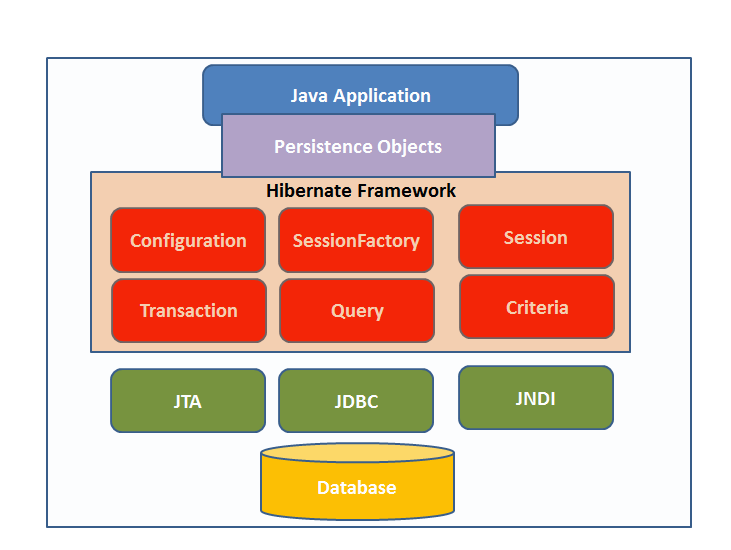
\includegraphics[scale=0.5]{hib-arch.png}%
\caption{Struttura di Hibernate}\label{fig:hibernate}%
\end{figure}

L'oggetto Configuration \`e di fondamentale importanza per il funzionamento del framework, in quanto contiene informazioni che riguardano:
\begin{itemize}
\item la connessione al database
\item il class mapping
\end{itemize}
la prima viene gestita mediante il file di configurazione \emph{hibernate.cfg.xml}, mentre il mapping tra le classi java e le tabelle del database, pu\`o avvenire mediante file di configurazione \textit{XML}, oppure, tramite l'inserimento diretto all'interno delle classi del codice inerente alla mappatura utilizzando lo stile Java Annotation.

\FloatBarrier
\begin{figure}[!htb]
\centering%
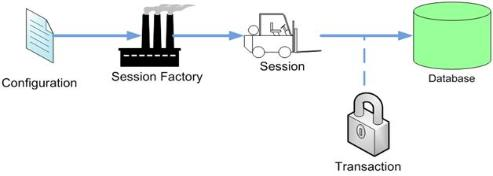
\includegraphics[scale=0.7]{hiber-arch2.jpg}%
\caption{Workflow Hibernate}\label{fig:hibernate2}%
\end{figure}

Questo oggetto viene creato una sola volta all'atto della inizializzazione della applicazione,

\begin{lstlisting}
Configuration config = new Configuration().configure("/it/resources/hibernate.cfg.xml");
\end{lstlisting}

e dopo che \`e stato utilizzato per la creazione di un altro oggetto, il SessionFactory, resta inutilizzato.

\begin{lstlisting}
SessionFactory sessionFactory = config.buildSessionFactory();
\end{lstlisting}

Quest'ultimo quindi, viene anch'esso creato una sola volta allo startup, ma a differenza di Configuration, viene utilizzato in tutta l'applicazione. L'oggetto SessionFactory \`e thread safe, ed \`e utilizzato da tutti i thread dell'applicazione, inoltre, siccome dipende da Configuration, che a sua volta si riferisce ad uno specifico database, potr\`a puntare solo a quel database. Nel caso di connessioni a database multipli, avremmo mulipli Configuration e quindi multipli SessionFactory, uno per ogni Configuration.
Il SessionFactory, come si evince dal nome, risulta essere uno stampo da cui creare gli oggetti Session, necessari ogni qualvolta occorre effettuare una interazione con il database. Quando con un oggetto di questo tipo viene aperta una sessione di lavoro,

\begin{lstlisting}
Session session = sessionFactory.openSession();
\end{lstlisting}

viene stabilita una connessione fisica con il database, e siccome non \`e thread safe, dopo aver effettuato le operazioni necessarie, occorre poi chiuderla manualmente, in modo da non mantenere connessioni aperte inutilmente.
Se durante una sessione di lavoro, occorre fare operazioni di modifica sul database, come inserimenti, aggiornamenti o cancellazioni, occorre gestirle come transazioni: a tal proposito l'oggetto Session viene a sua volta utilizzato per la creazione di oggetti Transaction. 
In Hibernate le transazioni sono gestite dal TransactionManager che permette allo sviluppatore di astrarsi dal livello sottostante (JDBC, JTA, ecc.) evitando di scrivere codice specifico. Infine Query e Criteria sono utilizzati per recuperare oggetti persistenti. Gli oggetti Query utilizzano SQL oppure HQL (Hibernate Query Language) per il recupero di dati dal database e per la creazione di oggetti, mentre Criteria utilizza oggetti per la costruzione e la esecuzione di una richiesta di recupero dati. 
